\section*{Valid-Invalid Protocol (write-through)}
\begin{minipage}{0.4\linewidth}
\begin{tikzpicture}[node distance=0.3cm]
  \node[recstate] (v) at (0,3) {Valid};
  \node[recstate, initial] (i) at (0,0) {Invalid};

  % invalid (start) --> valid
  \draw[->] (i) edge[ivp,bend left] node[above,sloped]{PrRd / BusRd} (v);
  % valid --> invalid
  \draw[->,densely dashed]
  (v) edge[ivp,bend left] node[above,sloped] {-- / BusWr} (i);
  % valid itself
  \draw[->] (v) edge[loop]
  node[left,xshift=-.5cm,rotate=40]{PrRd / --}    %node 1
  node[right,xshift=.5cm,rotate=-40]{PrWr / BusWr} %node 2
  ();
  % invalid itself
  \draw[->] (i) edge[in=-140,out=-40,loop] node[below]{PrWr / BusWr}();
\end{tikzpicture}
\end{minipage}
\begin{minipage}{0.6\linewidth}
  \flushleft
  \begin{itemize}
  \item Assume write-through, write-no-allocate
  \item \texttt{LDR} to fetch data from mem
  \item BusRd to request data from mem
  \item Bring data to cache: \textsf{Invalid} $\rightarrow$ \textsf{Valid}
  \item Additional Rds just uses data in cahce
  \item PrWr/BusWr writes to both cache\&mem
  \item Another proc may init a BusWr/-- (\texttt{--->})
  \item BusWr/-- broadcast to other caches
  \item All \textsf{Valid} caches $\rightarrow$ \textsf{Invalid}
  \item Only BusWr/-- init-er cache remains \textsf{Valid}
  \end{itemize}
  \begin{tabular}{l|l}
    \hline
    Short & Full Action \\
    \hline
    PrRd & Processor Read \\
    PrWr & Processor Write \\
    BusRd & Bus Read \\
    BusWr & Bus Write \\
    \hline
  \end{tabular}
\end{minipage}
\begin{minipage}[t]{0.5\linewidth}
  \flushleft
  \textsf{Valid} state:
  \begin{enumerate}
  \item data in cache is valid \emph{and}
  \item it matches corresponding data in main memory
  \item[] state means the \textbf{state of a cache line}
  \end{enumerate}
\end{minipage}
\begin{minipage}[t]{0.5\linewidth}
  \flushleft
  \textsf{Invalid} state:
    \begin{enumerate}
    \item data in cache is invalid because
    \item it either does not match corresponding data in main memory \emph{or} explicitly gets invalidated
    \end{enumerate}
\end{minipage}
\begin{itemize}
\item \textbf{PrRd/—} a processor read operation. If data is in \textsf{Valid} state,
the read operation $\rightarrow$ a hit and data is fetched from the cache.  If data is in \textsf{Invalid} state, the read operation $\rightarrow$ a miss and data is fetched from the main memory
\item \textbf{PrWr/BusWr} a processor write operation. In a write-through, writeno-allocate cache, data is written to both cache (if it’s in \textsf{Valid} state) and the main memory
\item \textbf{PrRd/BusRd} a processor read operation. It results in a miss
(because data in \textsf{Invalid} state).  Data is fetched from the main memory
and the cache state transitions to \textsf{Valid}
\item \textbf{BusWr/I—} a write operation initiated by another processor (or
device) on the bus.  The cache controller snoops the bus, detects that the write
operation affects the data in cache, and invalidates the cache line
\item \textbf{PrRd/BusRd} $\Rightarrow$ a processor read leads to a bus read action
\item generally, A/B $\Rightarrow$ if A is observed then B is generate
\item \verb|--| or -- means not available or irrelevant
\item Shared bus is atomic; Memory operations are atomic
\item Processor waits until prev mem op completed before issuing a new one
\item Invalidation happens during bus transaction (part of invalidation broadcast)
\end{itemize}
\begin{tabular}{lll|lll|l}
  \hline
  Core1 & State & Data* & Core2 & State & Data & Action \\
  \hline
  \texttt{LD 0xA} & \textsf{Valid} & 2 &&& & BusRd\\
  &&&\texttt{LD 0xA} & \textsf{Valid} & 2 & BusRd\\
  \hline
  \multicolumn{7}{l}{Additional \texttt{LD} from C1/C2 satisfied locally with PrRd only, no BusRd}\\
  \hline
  \multicolumn{7}{l}{Data is the value in both cache and at addr \texttt{0xA} in main memory}\\
  \hline
  \multicolumn{7}{l}{\texttt{ST} from C1 makes C2 cache \textsf{Invalid}; C1 cache remains \textsf{Valid}}\\
  \hline
  \texttt{ST 0xA} & \textsf{Valid} & 3 & & \textsf{Invalid} & 2 & BusWr\\
   & \textsf{Valid} & 3 & \texttt{LD 0xA} & \textsf{Valid} & 3 & BusRd\\
  \hline
\end{tabular}
\subsection*{Drawbacks}
\begin{itemize}
\item Every write updates cache and main memory (write-through)
\item Every write requires broadcast and snoop on shared bus (expensive)
\end{itemize}
\columnbreak
\section*{Modified-Shared-Invalid (MSI) Protocol}
\begin{minipage}{0.5\linewidth}
\begin{tikzpicture}[node distance=0.3cm]
  \node[recstate] (m) at (0,5) {Modified};
  \node[recstate] (s) at (0,2.5) {Shared};
  \node[recstate, initial] (i) at (0,0) {Invalid};

  % I (start) --> M
  \draw[->] (i) edge[msi,bend left]
  node[msinl,above,sloped,rotate=180]{\pro{PrWr/}\bus{BusRdX}} (m);
  % I --> S
  \draw[->] (i) edge[msi,bend left]
  node[msinl,above,sloped,rotate=-10,xshift=.3cm]{\pro{PrRd/}\bus{BusRd}} (s);
  % S --> M
  \draw[->] (s) edge[msi,bend left]
  node[msinl,below,sloped,rotate=180,yshift=-.1cm]{\pro{PrWr/}\bus{BusRdX}} (m);
  % M itself
  \draw[color=Brown,->] (m) edge[loop]
  node[msinl,left,xshift=-.5cm,rotate=40]{PrRd / --}  %node 1
  node[msinl,right,xshift=.5cm,rotate=-40]{PrWr / --} %node 2
  ();

  % M --> S
  \draw[->,densely dashed] (m) edge[msibs,bend left]
  node[msinl,above,sloped,color=RoyalBlue] {BusRd/BusWB} (s);
  % S --> I
  \draw[->,densely dashed] (s) edge[msibs,bend left]
  node[msinl,above,sloped,color=RoyalBlue,rotate=10,xshift=-.3cm] {BusRdX/--} (i);
  % M --> I
  \draw[->,densely dashed] (m) edge[msibs,bend left]
  node[msinl,above,sloped,color=RoyalBlue,rotate=180] {BusRdX/BusWB} (i);

  % S itself
  \draw[->,draw=Brown] (s) edge[in=-45,out=-135,loop]
  node[msinl,left,color=Brown,rotate=-20,yshift=-.2cm] {PrRd/--}
  node[msinl,right,color=RoyalBlue,rotate=20,yshift=-.2cm] {BusRd/--}
  ();
\end{tikzpicture}
\end{minipage}
\begin{minipage}{0.5\linewidth}
  % arrows
  % table
  \begin{itemize}
  \item \pro{brown lines} init-ed by processor
  \item \bus{blue lines} init-ed by bus
  \item \pro{A/}\bus{B} means A cause B
  \item \pro{PrRd} and \textsf{I} $\to$ \textsf{S} (read-only)
  \item \pro{PrWr} and \textsf{I} $\to$ \textsf{M} (exclusive)
    \begin{enumerate}
    \item action initer has exclusive access to this data addr
    \item it can read/write to addr freely and remain in \textsf{M}
    \item other caches in \textsf{S} or \textsf{M} all $\to$ \textsf{I}
    \end{enumerate}
  \item If any \pro{Pr} actions (left-side) causes a \bus{Bus} action, all other caches must follow the \bus{Bus} action (right-side) to update their states
  \end{itemize}
  \begin{tabular}{l}
    \hline
    Processor Read (PrRd)\\
    Processor Write (PrWr)\\
    Bus Read (BusRd)\\
    Bus Read Exclusive (BusRdX)\\
    Bus Writeback (BusWB/Flush)\\
    \hline
  \end{tabular}
\end{minipage}
\begin{itemize}
\item \textsf{M}odified (dirty/exclusive), only this cache has a valid copy
of the cache line, and the copy in main memory is stale
\item \textsf{S}hared: the cache line is in unmodified state in this cache, main
memory is up-to-date, and 0/more caches may also have an up-to-date copy
\item \textsf{I}nvalid: Not present or already invalidated by a bus request
\item \bus{BusRd}: cache ctrler obtains cache line copy with no intent to
modify
\item \bus{BusRdX} cache ctrler obtains \emph{exclusive} copy and intends to modify; main memory supplies the data and all other caches are invalidated
\item \bus{BusRdx/BusWB(Flush)}: processor unaware of it and not expect a response. Main memory is updated with the latest content
\item MSI lets caches serve writes without updating memory so main memory can have \emph{stale} (outdated) data
\item When both cache and memory responds to Rd, cache must override response from main memory
\item Corollary rule: Before a shared/invalid copy can be written and placed in \textsf{M}, all other potential copies must be invalidated via a \bus{BusRdX}
\end{itemize}
\begin{tabular}{p{0.5cm}|lcc|lcc|p{1.8cm}}
  \hline
  Time & Core1 & State & Data & Core2 & State & Data & \pro{A}/\bus{B} \\
  \hline
  $T_1$ & \texttt{LD 0xA} & \textsf{I}$\to$\textsf{S} & $\to$2 && -- & -- & {\footnotesize\pro{PrRd/}\bus{BusRd}}\\
  \hline
  $T_2$ && \textsf{S} & 2 &\texttt{LD 0xA} & \textsf{I}$\to$\textsf{S} & $\to$2 & {\footnotesize\pro{PrRd/}\bus{BusRd}}\\
  \hline
  $T_3$ & \texttt{ST 0xA} & \textsf{S}$\to$\textcolor{red}{\textsf{M}} & 2$\to$\textcolor{red}{3} & & \textsf{S}$\to$\textsf{\color{red}I} & $\to$2 & {\footnotesize\pro{PrWr/}\bus{BusRdX}}\\
  \hline
  $T_4$ & & \textsf{M}$\to$\textcolor{red}{\textsf{I}} & 3 & \texttt{ST 0xA} & \textsf{I}$\to$\textcolor{red}{\textsf{M}} & 2$\to$\textcolor{red}{10} & {\footnotesize\bus{BusRdX/BusWB}}\\
  \hline
  $T_5$ & \texttt{LD 0xA} & \textsf{I}$\to$\textcolor{red}{\textsf{S}} & \textcolor{red}{10} &  & \textsf{M}$\to$\textcolor{red}{\textsf{S}} & 10 &{\footnotesize\bus{BusRd/BusWB}} \\
  \hline
\end{tabular}
\begin{itemize}
\item After $T_2$, additional \texttt{LD} from Core1/2 satisfied locally without \bus{BusRd}
\item At $T_3$, Core2 invalidates its cache state and Core1 trans to \textsf{M} and updates data in its cache \emph{only}; \emph{no} write/update to main memory (write-back cache)
\item After $T_3$, additional \texttt{LD}/\texttt{ST} from Core1 satisfied locally, without bus transactions
\item At $T_4$, Core1 inits a \bus{BusWB(Flush)} first (taking value in its cache 3 and write back to main memory at \texttt{0xA}) and also trans from \textsf{M} to \textsf{I}
\item At $T_4$, after Core1 done the above, Core2 inits \bus{BusRdX}, trans to \textsf{M}, and updates data in its cache to 10
\item At $T_5$, Core1 inits \bus{BusRd} which cause Core2 to first do \bus{BusWB}: writes 10 to main memory at \texttt{0xA} and trans to \textsf{S}
\end{itemize}
\subsection*{Drawbacks and solution (use MESI)}
\begin{itemize}
\item 2 bus transactions for every read-modify-write of private data
\end{itemize}
\columnbreak

\section*{Modified-Shared-Exclusive Invalid (MESI) Protocol}
\begin{tikzpicture}[node distance=0.3cm]
  \node[recstate] (m) at (0,7.5) {Modified};
  \node[recstate] (e) at (0,5) {Exclusive};
  \node[recstate] (s) at (0,2.5) {Shared};
  \node[recstate, initial] (i) at (0,0) {Invalid};

  % I (start) --> M
  \draw[->] (i) edge[msi,bend left]
  node[msinl,above,sloped,rotate=180]{\pro{PrWr/}\bus{BusRdX}} (m);
  % I --> E
  \draw[->] (i) edge[msi,bend left]
  node[msinl,above,sloped,rotate=180,xshift=.3cm,yshift=-.1cm]
  {\pro{PrRd/}\bus{BusRd($\overline{S}$)}} (e);
  % I --> S
  \draw[->] (i) edge[msi,bend left]
  node[msinl,above,sloped,rotate=-10,xshift=.4cm,yshift=-.1cm]
  {\pro{PrRd/}\bus{BusRd(S)}} (s);
  % S --> M
  \draw[->] (s) edge[msi,bend left]
  node[msinl,below,sloped,rotate=175,xshift=.5cm]
  {\pro{PrWr/}\bus{BusRdX}} (m);
  % E- --> M
  \draw[->] (e) edge[msi,bend left]
  node[msinl,below,sloped] {\pro{PrWr/}\bus{--}} (m);
  % M itself
  \draw[color=Brown,->] (m) edge[loop]
  node[msinl,left,xshift=-.5cm,rotate=40]{PrRd / --}  %node 1
  node[msinl,right,xshift=.5cm,rotate=-40]{PrWr / --} %node 2
  ();

  % M --> S
  \draw[->,densely dashed] (m) edge[msibs,bend left]
  node[msinl,above,sloped,color=RoyalBlue] {BusRd/BusWB} (s);
  % E --> S
  \draw[->,densely dashed] (e) edge[msibs,bend left]
  node[msinl,above,sloped,color=RoyalBlue] {BusRd/BusWB} (s);
  % E --> I
  \draw[->,densely dashed] (e) edge[msibs,bend left]
  node[msinl,below,sloped,color=RoyalBlue,xshift=.3cm]
  {BusRdX/BusWB} (i);
  % E itself
  \draw[->] (e) edge[msi,loop,color=black] node[msinl] {PrRd/--} ();

  % S --> I
  \draw[->,densely dashed] (s) edge[msibs,bend left]
  node[msinl,above,sloped,color=RoyalBlue,rotate=10,xshift=-.3cm,yshift=-.1cm]
  {BusRdX/BusWB} (i);
  % M --> I
  \draw[->,densely dashed] (m) edge[msibs,bend left]
  node[msinl,above,sloped,color=RoyalBlue,rotate=180,xshift=-.2cm]
  {BusRdX/BusWB} (i);

  % S itself
  \draw[->,draw=Brown] (s) edge[in=-45,out=-135,loop]
  node[msinl,left,color=Brown,rotate=-35,yshift=-.3cm] {PrRd/--}
  node[msinl,right,color=RoyalBlue,rotate=35,yshift=-.4cm,xshift=-.6cm]
  {BusRd/BusWB}
  ();

  % text node
  \draw[xshift=2.8cm,yshift=4cm]
  node[right, text width=3cm] {
    \begin{itemize}
    \item \textsf{\textbf{E}}xclusive (exclusive-clean): only one cache (this cache) has a copy of the cache line and it has not been modified (main memory is up-to-date)
    \item \textsf{\textbf{S}}hared: potentially two or
    more processors have this block in their cache in
    an unmodified state.
  \item \textcolor{RoyalBlue}{\textsf{BusRd($\overline{\textsf{S}}$)}} means no other sharers and thus exclusive read: \textsf{I}$\to$\textsf{E}
  \item \textcolor{RoyalBlue}{\textsf{BusRd(S)}} means with other sharers and thus shared read: \textsf{I}$\to$\textsf{S}
  \item \textsf{M} and \textsf{I} are same as in MSI
    \end{itemize}
  };
\end{tikzpicture}
\begin{itemize}
\item if no other sharers, a read acquires cache line in \textsf{E} instead of \textsf{S}
\item writes silently cause \textsf{E} $\to$ \textsf{M} (exclusive, dirty) without bus trans
\end{itemize}
\subsection*{Director-Based Cache coherence (larger systems)}
Route all coherence transactions through a directory
\begin{itemize}
\item tracks contents of private caches (send coherence messages to L2s which contain the line)
\item no broadcasts (a dedicated process works on tracking)
\item serves as ordering point for conflicting requests $\to$ unordered networks
\item 5-stage MOESI, MESIF allow for cache-to-cache transfers
\end{itemize}
\subsection*{Cache line Design}
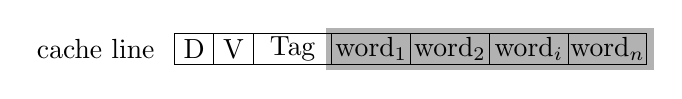
\begin{tikzpicture}
  \node[] (d) at (.25,0.2) {D};
  \node[] (v) at (.75,0.2) {V};
  \node[] (t) at (1.5,0.2) {Tag};
  \node[fill=gray!60] (w1) at (2.5,0.2) {word$_1$};
  \node[fill=gray!60] (w2) at (3.5,0.2) {word$_2$};
  \node[fill=gray!60] (wi) at (4.5,0.2) {word$_i$};
  \node[fill=gray!60] (wn) at (5.5,0.2) {word$_n$};
  \node[] (lb) at (-1,0.2) {cache line};
  \draw (0,0) rectangle (6,.4);
  \draw (.5,0) -- (.5,.4);
  \draw (1,0) -- (1,.4);
  \draw (2,0) -- (2,.4);
  \draw (3,0) -- (3,.4);
  \draw (4,0) -- (4,.4);
  \draw (5,0) -- (5,.4);
\end{tikzpicture}
\begin{itemize}
\item \textsf{D} (dirty) bit.  If $D=1$, data in cache modified and needs to be written back to main memory before eviction; if $D=0$, data clean and can be safely evicted without write-back
\item \textsf{V} (valid) bit.  If $V=1 \to$ data in cache line valid; if $V=0 \to$ cache line is empty or invalidated (should \emph{not} be read)
\item Tag bits contain the memory addr where the data is read from or written back to
\end{itemize}
\subsection*{False Sharing (severely affect parallel performance)}
\begin{itemize}
\item Condition where 2 processors write to different memory addresses but the addresses map to the same cache line
\item Suppose P$_1$ works on word$_j$ and P$_2$ works on word$_k$ (word$_j$ and word$_k$ are in the same cache line)
\item Each time $P_1$ or $P_2$ writes will (unnecessarily) invalidate the line and cause the other to wait for cache coherence; such ``ping-pong'' interactions cause high serialization overhead
\item use padding to alleviate the situations: P$_1$ pads its data so that the data with padding take up an entire cache line
\end{itemize}
